\chapter{Linear Time-Invariant Systems}

\section{Time Invariance}
In Linear Time-Invariant (LTI) Systems, we consider time-domain signals, such as continuous-time signals (whose time domain is $\mathbb{R}_+$) and discrete-time signals (whose time domain is $\mathbb{Z}_+$).
Then, systems with continuous-time input and output signals are called continuous-time systems, and systems with discrete-time input and output signals are called discrete-time systems.
A simple example of a continuous-time system would be a delay system, where it receives an input signal and outputs another signal that is a delayed version of the input:
\[
    \forall t \in \mathbb{R}, y(t) = x(t - \tau)
\]
But this simple continuous-time system becomes critical in the definition of ``time-invariance''.
Particularly, if a system is time-invariant, then the system's output signal upon receiving a delayed input must be equivalent to the delayed version of system's output signal on the original input signal:
\[
    \forall \tau \in \mathbb{R}, S \circ D_\tau = D_\tau \circ S
\]
In other words:
\[
    S(D_\tau (x)) = D_\tau (S(x))
\]
A visual summary of this phenomenon follows:
\begin{center}
    \begin{figure}[h]
        \centering
        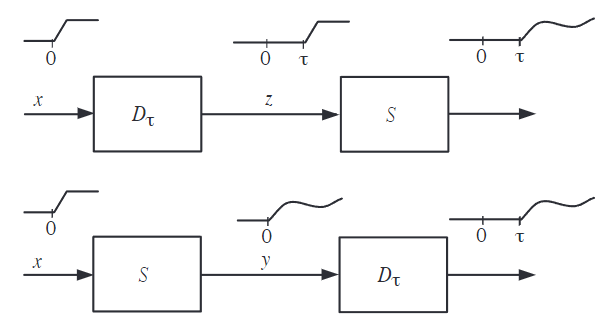
\includegraphics[width=0.7\textwidth]{figs/ln13/time-invariant.png}
        \caption{In time-invariant systems, the system's output from a delayed signal is equal to the delayed system's output of original input.}
    \end{figure}
\end{center}
In another interpretation, we may say that a time-invaraint system $S$ (whose output signal is $y$) receives a delayed input $D_\tau (x)$ and outputs an equivalently delayed output $D_\tau(y)$.
This preservation, or invariance, of shifting in signals is otherwise known as ``shift invariance''.

\section{Linearity of System}
Remember from before that we have defined the linearity of a functino as the intersection of two distinct conditions: superposition and homogeneity:
\[
    \begin{cases}
        (ax)(t) = a(x(t)) \\
        (x_1 + x_2)(t) = x_1(t) + x_2(t)
    \end{cases}
\]
The lineraity of a complex system (systems that map complex-valued functions to complex-valued functions, $S: [\mathbb{C} \rightarrow \mathbb{C}] \rightarrow [\mathbb{C} \rightarrow \mathbb{C}]$) is similarly defined to be the intersection of two conditions:
\[
    \begin{cases}
        (aS)(t) = a(S(t)) \\
        (S_1 + S_2)(t) = S_1(t) + S_2(t)
    \end{cases}
\]

\section{Linearity and Time-Invariance}
Both linearity and time-invariance are realistically fictional properties; that is, they are usually ``ideal properties'' of electronic systems that are not realistically satisfied.
The combination of these useful proeprties provide linear time-invariant systems, which presents the two following simple behaviors:
\begin{enumerate}
    \item Given a sinusoid at the input, the output of an LTI system will be a sinusoid with the same frequency (due to linearity), but possibly with different phase and amplitude (as results of linear transformations, or time-invariance).
    \item Given a weighted sum of sinusoids as an input, the output is a sum of sinusoids with the same frequencies, but possibly different phases and amplitudes.
\end{enumerate}
The most mysterious aspect of the above behavior depiction is perhaps the reason at which phases change. This comes back to a previously introduction of complex exponential expressions for trigonometric functions:
\[
    \forall t \in \mathbb{R}, x(t) = e^{i \omega t} = \cos(\omega t) + i \sin{\omega t}
\]
Under such rule, a delated system's complex exponential expression follows:
\[
    \forall t \in \mathbb{R}, \tau \in \mathbb{R}, x(t - \tau) = e^{i \omega (t - \tau)} = e^{i \omega t} e^{-i \omega \tau}
\]
so the time-invariance of LTI systems allow for delayed inputs, which can lead to the phase changes in a LTI system's output signal from its inputs.

When the output of a system is only a scaled version of the input, the input is called an \textbf{eigenfunction}.
This bodes similarity to eigenvectors in a linear algebra context: while an eigenvector results from a transformation $A$ on a vector $\vec{v}$ that leads to a scaled version of $\vec{v}$, an eigenfunction results from a transformation (system) $S$ that leads to a scaled version of the transformed functions.
Eigenfunctions are convenient in the sense eigenvectors are.

And interestingly, complex exponentials are eignefunctions of LTI systems.
Provided an LTI system,
\[
    \forall t, \tau \in \mathbb{R}, y(t - \tau) = e^{-i \omega \tau} y(t)
\]
At $t = 0$, we see:
\[
    \forall \tau \in \mathbb{R}, y(-\tau) = e^{-i \omega \tau} y(0)
\]
At where $t = -\tau$, $y(t) = e^{i \omega t} y(0)$.
With this transformation $t = -\tau$, we discover that $y(t)$ is an eigenfunction of $e^{i \omega t}$ scaled by $y(0)$, which doesn't depend on time.
Still, we can further discover that this function $y(0)$ does depend on $\omega$ in general, as it is the output evaluated at timestep $0$ provided some input $e^{i \omega t}$.
\[
    \forall \omega \in \mathbb{R}, H(\omega) = y(0) = (S(x))(0), \text{where} \forall t \in \mathbb{R}, x(t) = e^{i \omega t}
\]
Substituting this back to the first expression of this paragraph:
\[
    y(t) = H(\omega) e^{i \omega t}
\]
when the input is $e^{i \omega t}$ and $H(\omega)$ is a function of $\omega \in \mathbb{R}$ (the frequency of the input complex exponential).
Therefore, outside of the argument of our output signal $t$, another moving part to the output of $y(t)$ becomes the frequency of our input signal: $\omega$.
Following such logic, we define for every LTI system a ``frequency response'':
\begin{ln-define}{Frequency Response}{}
    The function $H: \mathbb{R} \rightarrow \mathbb{C}$ is called the frequency response, which defines the response of any LTI system to a complex exponential input at some given frequency, and gives the scaling factor of the system's eigenfunction.
\end{ln-define}
